\documentclass[11pt]{article}

\usepackage{mathtools}
\usepackage{amssymb}
\usepackage{amsmath}
\usepackage{amsthm}
\usepackage{hyperref}
\usepackage{microtype}
\usepackage{graphicx}
\graphicspath{ {./img/} }

\setlength{\parindent}{0cm}
\let\emptyset\varnothing

\title{\textbf{CSCI/MATH 2113 Discrete Structures} \\ 6.3 - 6.4 Finite State Machines and Mealy Machines}
\author{Alyssa Motas}

\begin{document}

    \maketitle

    \pagebreak

    \tableofcontents

    \pagebreak

    \section{Finite State Machine}

    A \emph{finite state machine} is a five-tuple \[M = (S, \mathcal{I}, \mathcal{O}, v, w)\] where 
    \begin{itemize}
        \item \(S\) is the set of internal states for $M$,
        \item \(\mathcal{I}\) is the input alphabet for $M$,
        \item \(\mathcal{O}\) is the output alphabet for $M$,
        \item \(v: S \times \mathcal{I} \rightarrow S\) is the next state function,
        \item \(w: S \times \mathcal{I} \rightarrow \mathcal{O}\) is the output function.
    \end{itemize}

    \subsection{Example}

    Let \(M = (S, \mathcal{I}, \mathcal{O}, v, w)\) with \(S = \{s_0, s_1, s_2\}\), \(\mathcal{I} = \mathcal{O} = \{0,1\}\) and $v$ and $w$ are defined as

    \begin{center}
        \begin{tabular}{| c | c | c |} \hline
              &         $v$         &  $w$ \\ \hline
              & 0     \quad 1       & 0 \quad 1 \\ \hline
        $s_0$ & $s_0$ \quad $s_1$   & 0 \quad 0 \\ 
        $s_1$ & $s_2$ \quad $s_1$   & 0 \quad 0 \\
        $s_2$ & $s_0$ \quad $s_1$   & 0 \quad 1 \\ \hline
        \end{tabular}
    \end{center}

    On input 1010, starting in state \(s_0\), the output is 0010:
    \begin{center}
        \begin{tabular}{| c | c | c | c | c | c |} \hline
                   & $t_0$              & $t_1$            & $t_2$            & $t_3$            & $t_4$ \\ \hline
            State  & $s_0$              & $v(s_0,1) = s_1$ & $v(s_1,0) = s_2$ & $v(s_2,1) = s_1$ & $v(s_1,0) = s_2$ \\
            Input  & 1                  &   0              &   1              &   0              &   0  \\
            Output & $w(s_0,1) = 0$     & $w(s_1,0) = 0$   & $w(s_2,1) = 1$   & $w(s_1,0) = 0$   &   -   \\ \hline
        \end{tabular}
    \end{center}

    \pagebreak

    \section{State diagrams}

    Since we are primarily interested in the output, not in the sequence of transition states, the same machine can be represented by means of a \emph{state diagram}. In such a diagram, each internal state $s$ is represented by a circle with $s$ inside of it. For states \(s_i,s_j\), if \(v(s_i,x) = s_j\) for \(x \in \mathcal{I}\), and \(w(s_i,x) = y\) for \(y \in \mathcal{O}\), we represent this by drawing a \emph{directed edge} from the circle for \(s_i\) to the circle for \(s_j\) and labeling the arc with the inptu $x$ and output $y$.

    \begin{center}
        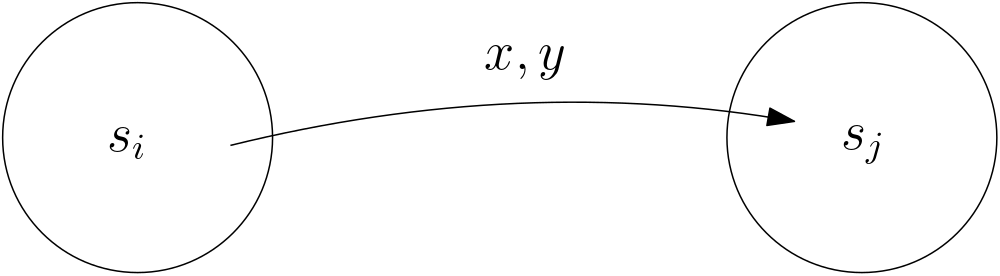
\includegraphics[width=10cm]{figure.png}  
    \end{center}

    The previous example becomes

    \begin{center}
        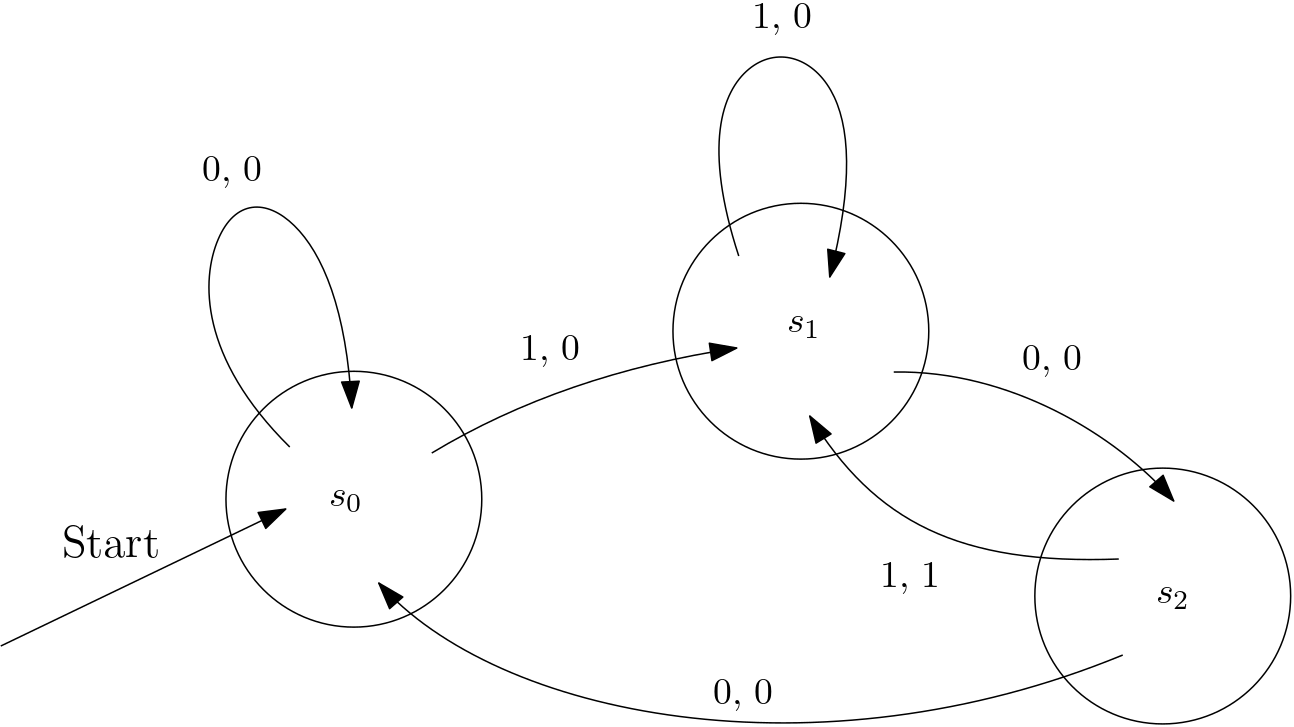
\includegraphics[width=10cm]{figure2.png}
    \end{center}

    We can think of a machine (such that \(\mathcal{I} = \mathcal{O}\) as associating words over \(\mathcal{I}\) to other words over \(\mathcal{I}\). Hence, a machine represents a relation on \(\mathcal{I}^*\).
   
\end{document}